\chapter{Introduction}

Definition by NIST:

\begin{itemize}
    \item On-Demand self service: get resources without human intervention
    \item Broad network access: accessible with multiple devices
    \item Resource pooling: physical/virtual resources dynamically assigned and according to consumer demand
    \item Rapid elasticity: shrink and grow capacity
    \item Measured services: monitor/control/report resources usage transparently
\end{itemize}

\section{Cloud models}

There are 3 main cloud service models: SaaS, PaaS, IaaS

\subsection{Software-as-a-Service (SaaS)}

”Ready-to-wear” application hosted by a vendor on the cloud. This is the main cloud computing market. There are multiples advantages: little or no administration, access anywhere, compatibility, collaborative applications. But also a few disadvantages: vendor lock-in and costs. Business: \textit{saleforce.com}, \textit{slack}, office and consumers: \textit{gmail}, \textit{instagram}.

\subsection{Platform-as-a-Service (PaaS)}

Hosting of managed operation system, associated environment and services by a vendor: deployment and configuration, databases, web servers, identity management, programming environment and libraries. The target is application developers

\subsection{Infrastructure-as-a-Service (IaaS)}

Hosting servers and resources that target IT infrastructure managers and developers. They provides virtualized equivalent of IT resources: VM, storage, network. They have flexibility, full control and privacy but need maintenance and they are complex.

\section{Types of clouds}

\subsection{Public clouds}

Services rendered on a data center owned by a third-party company. Over a public network. The infrastructure is shared with other client: pay-per-use model, no maintenance or management cost. There are multiples security and privacy considerations: leaks due to attacks ? legal consideration: is the NSA allowed to access my file ? We need to trust cloud provider with security enforcement.

\subsection{Private clouds}

Services rendered on a data center owned by a third-party company. Over a public network. The infrastructure is shared with other client: pay-per-use model, no maintenance or management cost. There are multiples security and privacy considerations: leaks due to attacks ? legal consideration: is the NSA allowed to access my file ? We need to trust cloud provider with security enforcement.

\subsection{Hybrid Clouds}

Composition of private and public: multi-site deployment, services available only in one provider, cost effectiveness. Cloud bursting: temporary capacity offloading from private to public cloud. Hybrid processing of sensitive/non-sensitive data but operation and integration more complex.

\chapter{Virtualization}

\section{Machine virtualization}

Virtualization abstracts resources to users and applications from physical resources. This allows a decoupled management of a large set of virtual cloud services and a large set of physical machines supporting them. This provide flexibility, isolation and dependability, this is also cost-efficiency.

\subsection{Basic}

For now, we only know one OS with multiple processes and applications. It cannot let each process access resources as it pleases. All processes must use memory, IO, processor. The resources are virtualize by the OS such as virtual memory. There are policies to arbitrate between demands.

A virtualized system is one physical computer who supports multiple virtual one, sharing resources between OS and applications. In 2014, there are more virtualized than non-virtualized servers.

Advantages for:
\begin{itemize}
    \item Users
    \begin{itemize}
        \item Resource abstraction and isolation
        \item Deploy-on-demand
        \item Enables the pay-as-you-go model
    \end{itemize}
    \item Cloud operators
    \begin{itemize}
        \item Reduces operational cost
        \item Larger and more efficient servers supporting
    \end{itemize}
\end{itemize}

There are also disadvantages: the cost of multiple OS state and maintenance, the performance penalty.

\subsection{Virtualization implementation}

There are two instruction modes in a machine virtualization context:
\begin{itemize}
    \item Non-privileged instructions still execute normally
    \item Privileged instructions: some trap to guest OS/virtualization layer
\end{itemize}

in this context, the hypervisor can emulate the behavior of unshared hardware.

\begin{figure}[H]
    \centering
    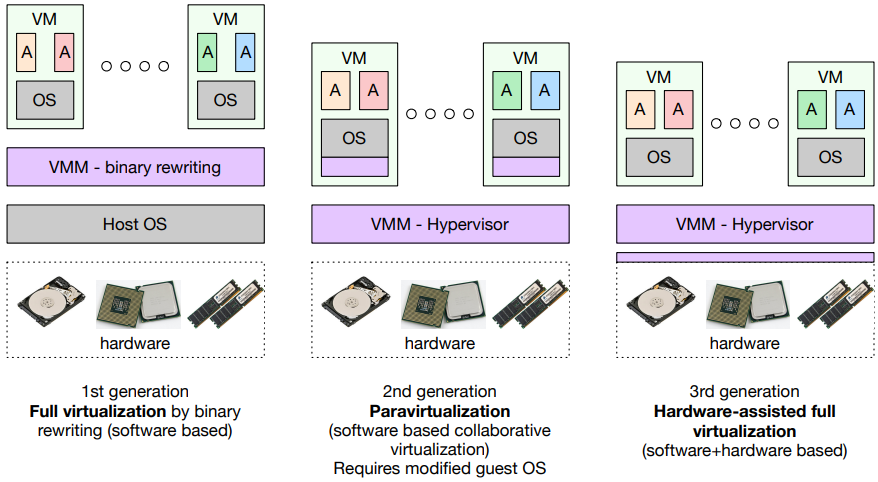
\includegraphics[width=0.8\textwidth,keepaspectratio]{virtualization}
\end{figure}

\subsubsection{First-generation virtualization}
Full by binary rewriting Emulation layer in host operating system. All the hardware is emulated including the CPU. Guest OS is not aware it is in an emulated environment.

\textbf{Pros}: Good VM isolation, good control of VM resource usage and total VM portability.

\textbf{Cons}: huge performance penalty, due to the privileged mode not being available to guest VM, must emulate it in software.

\subsubsection{Second-generation virtualization}
Paravirtualization Guest OS is modified ; no need to run privileged instructions itself, knows how to ask the hypervisor to handle operations that require privileges. Paravirtualized device drivers know how to efficiently address devices directly through hypervisor.
The hypervisor arbitrates between guest OSes

\textbf{Pros}: performance, OS awareness of virtualization allows inter-VM collaboration.

\textbf{Cons}: Requires OS vendor to provide paravirtualization-enabled version. Alternative: provide paravirtualization only partially through drivers (Microsoft Windows enlightenment’s, VirtualBox guest additions, etc.).

\subsubsection{Third-generation virtualization}
Full \& hardware-assisted Requires processor extensions such as Inter-VT or AMD-V (now everywhere), can intercept and emulate privileged operations in the guest OS in hardware (no need for host OS). The hypervisor is still in charge of resource allocation.

\textbf{Pros}: can run unmodified OS.

\textbf{Cons}: unmodified OS is not aware of virtualization, drivers code trigger lots of traps which kill performance. Therefore, you still need paravirtualized device drivers for performance $\Rightarrow$ hybrid virtualization.

\subsection{Virtualization and security}

\begin{itemize}
    \item Hypervisor-based rootkits: could be installed on non-virtualized systems, taking advantage of hardware-assisted virtualization. Successful rootkit can get higher privilege level than kernel and be almost impossible to detect.
    \item Collocation attacks: exploiting security flaws at the hypervisor level from one VM to inspect state of other VM. Exploiting data remaining in CPU cache after VM switch.
\end{itemize}

The hypervisor is \textbf{critical}.

\section{IaaS}

A service model allowing clients to rent resources from the cloud such as virtual machines (VM), virtual networks (VN) or storage. The user is in charge of installing and managing the OS and environment.

\textbf{Key players}: Amazon web services, Windows Azure, HP Converged Infrastructure, Google Compute Engine, Rackspace, IBMSmartCloud.

\subsection{Operations}

\begin{itemize}
    \item Allocate a resource on demand
    \item Deploy an image onto a host and in some cases: migrate VM between hosts, change a VM configuration dynamically
    \item Obtain configuration information (IP address)
    \item Manage access keys (SSH)
\end{itemize}

\subsection{Defining needs: instances}

Users need to define the capacity of the VM they want to use: Virtual CPUs (VCPU) and memory. Type of storage (remote or dedicated on the host).

\subsubsection{Rackspace example on Linux instances}

\begin{itemize}
    \item General purpose: 1 to 8 VCPUs, 1 to 8Gb ram and to 160Gb SSD
    \item Compute optimized: 2 to 32 VCPUs, 4 to 32Gb ram, no SSD
    \item I/O optimized: 4 to 32 VPCUs, 4 to 32Gb ram, 40Gb systems SSD + 150 to 1200Gb data SSD, high redundant bandwidth
    \item Memory optimized; 2 to 32 VPCUs, 15 to 240Gb ram, high redundant bandwidth
\end{itemize}

\subsubsection{Pricing}

In general, there are 3 pricing : for the server, the storage and the network. The server cost is per hour per VM, the storage cost is per GB per month and the network cost is per GB and depend if the flux is IN or OUT.

\subsection{How is the fleet managed}

A data center is a very complex infrastructure. Many operations are in common between IaaS so there is an IaaS managements system. Some are open-source like \textit{OpenStack} or \textit{OpenNebula}. there is also commercial offerings like \textit{Nutanix}.

We can do an analogy with an OS. We can considered IaaS management platforms as Cloud operating system as their role is similar in many ways.
\begin{itemize}
    \item Run VMs instead of processes
    \item Allocate fixed portions of RAM to different VMs instead of allocation using virtual memory
    \item Inter-VM networking vs. IPD
    \item Naming and configuration
    \item Authentication, protection and security
\end{itemize}

\subsubsection{Direct infrastructure access}

\begin{figure}[H]
    \centering
    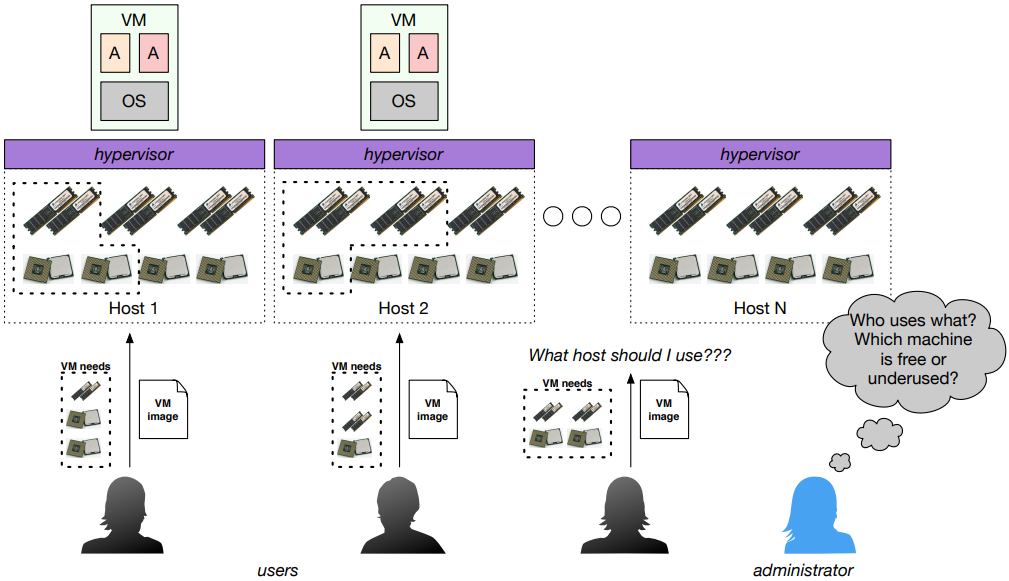
\includegraphics[width=0.8\textwidth,keepaspectratio]{direct_infrastructure_access}
\end{figure}

\subsubsection{IaaS management platform}

\begin{figure}[H]
    \centering
    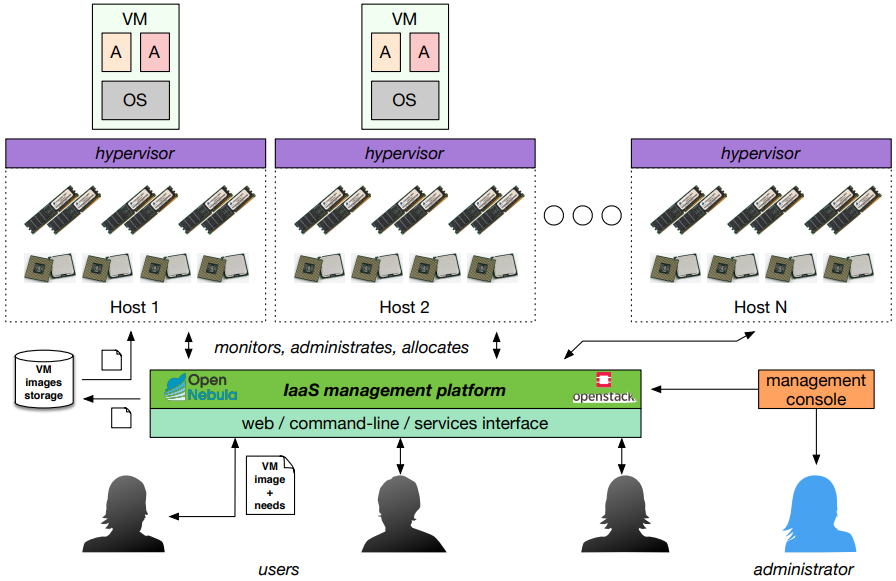
\includegraphics[width=0.8\textwidth,keepaspectratio]{management_platform}
\end{figure}

\section{Containers}

\begin{wrapfigure}[11]{r}{0.25\textwidth}
    \centering
    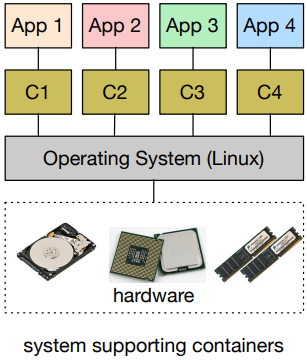
\includegraphics[width=\linewidth]{sys_containers}
\end{wrapfigure}

Instead of virtualizating a machine, we virtualize the OS. That allows the independent management of containerized applications. Machine virtualization decouples OS from hardware vs. containers who decouple application from OS. From Machine-oriented to an application oriented data-center.

\subsubsection{Requirements}

\begin{itemize}
    \item A single OS: multiple user-space instances over a single kernel-space instance
    \item Enabling mechanism = Isolation: No access or visibility across user-space instances (no sharing at all); processes in one user-space instance believe that they have the machine just for themselves. $\Rightarrow$ Linux's namespaces
    \item Enabling policy = resource management: Limit the use of resources by one container such as memory use, network use, disk quotas, etc. $\Rightarrow$ Linux's control groups (cgroups)
\end{itemize}

\subsubsection{Containers vs VM}

\begin{itemize}
    \item OS-level vs. machine virtualization: boundary = system call interface vs. hardware emulation
    \item Less overheads: system calls in kernel modified to handle different "contexts", resource allocation and monitoring require little resources
    \item Less flexibility: no support for arbitrary environment, unless specific emulation in place
    \item Isolation is not as good as with VMs: attack surface (Kernel system calls) larger than hypervisor attack surface, some resources (level-3 caches in CPU) not isolated
\end{itemize}

The best of both worlds: combine virtual machines and containers: decouple hardware and OS management (cloud/tenant), decouple OS and applications management (applications/tenant).

\begin{figure}[H]
    \centering
    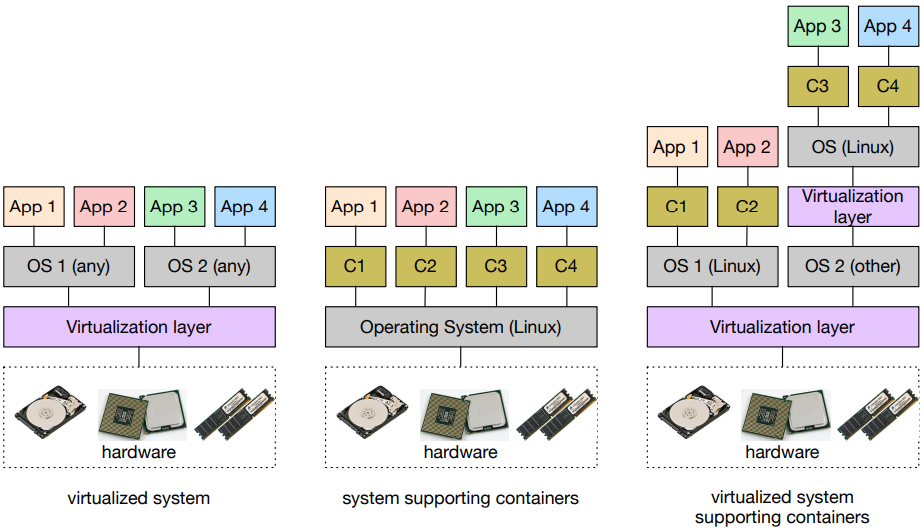
\includegraphics[width=0.8\textwidth,keepaspectratio]{vm_containers}
\end{figure}

\subsubsection{Linux containers}

Generic name for containers for Linux based on namespaces and cgroups. There are many of them like OpenVZ, LXC, Linux-VServer, Open Container Initative runC, Rocker by CoreOS. All of them are generally considered as relatively complex to use, configure and automate. Docker comes and simplifies these aspects.

\subsection{Docker}

Wrap-up complete applications inside containers. The file system contains everything needed to run the application : Runtime, system tools, and system libraries. This solve the portability problem of earlier implementation of the container concept, which assumed the same complete OS distribution. Docker offers full functional toolset including mechanisms for creating and manipulating portable containers : even if OS different in dev/testing/prod, linked to and used by the DevOps movement

\subsubsection{Running a first container and commands}

\begin{minted}[linenos, breaklines]{bash}
docker run -i -t ubuntu /bin/bash
    -i -t interactive shell with STDIN kept open
    ubuntu : base image
    /bin/bash : command to run after the creation
\end{minted}

You can logout with exit or ctrl-d
\begin{minted}[linenos, breaklines]{bash}
docker run ( eq . to docker create + docker start )
    -d : no shell
docker ps
    -a : all containers , running and stopped ones
    -l : latest running container
docker start [ identifier ]
    identifier can be the UID (e.g., f6a228e12606), the automaticallygenerated name (e.g., hardcore_rosalind) or the name provided
    to docker run with the --name option
docker attach
    re-attach to an interactive session
docker stop | kill
    send SIGSTOP or SIGKILL to container
docker inspect [identifier]
    get details about a running container
docker logs
docker images
    list locally-stored images
\end{minted}

\paragraph{Content of a docker image}
Made of filesystems layered over each other: it is called ”Union mount”, read only (bootfs is Linux boot filesystem, rootsfs is base OS filesystem), new readwrite FS on top when instantiated.

Copy-on-write approach: modified files copied in writeable container, reads go down layers until file found. The same base read-only FS is shared across containers on the same host.

\paragraph{Create an image}
Requires writing a DockerFile and running docker build in the same directory. We can publish images for free in Docker Hub. Here are some commands for Dockerfile:
\begin{minted}[linenos, breaklines]{bash}
CMD
    Command to run when launching the container
        Can be overridden by docker run argument
        If you do not want this , use ENTRYPOINT instead
WORKDIR / ENV / USER
    Set working directory , environment variables , user
ADD dir
    Copy files from build environment or URL
VOLUME
    Specific directory that will be outside the union file system and can be shared with other containers , even when not running
    Allow sharing data between containers
\end{minted}

\subsection{Composing and orchestrating containers}

Managing individual containers by hand and "wiring" them together can be a complex process: composition: group several containers together as a single entity. Example: web server + database + administration interface.

Managing the execution of a fleet of containers is also complex: coordination between multiple Docker hosts, resources management, service discovery, scheduling of the execution of multiple containers.

Some tools in Docker for managing sets of containers:
\begin{itemize}
    \item Docker compose: simple container composition
    \item Consul: service discovery
    \item Docker Swarm: orchestration and scheduling across multiple hosts
    \item Kubernetes:: large-scale orchestration and scheduling
\end{itemize}

\subsubsection{Docker-compose}

Described in a YAML file: lists the containers images to instantiate with the commands to run, the ports to instantiate/export and the volumes. Describe how they are linked : Container A links container B = Ports exported by B available for use from A. Service in container B named as “B” from A. Automatic setup of Docker network between A and B. To run it, we use docker-compose up that reads the YAML file docker-compose. yml in the same directory. Many docker commands have their compose equivalent.

\textbf{Example of a Dockerfile:}
\begin{minted}[linenos, breaklines]{bash}
web:
    image: ccs/composeapp
    command: python app.py
    ports:
        - "5000:5000"
    volumes:
        - .:/composeapp
    links:
        - redis
redis:
    image: redis
\end{minted}

\subsubsection{Docker swarm}

Managing multiple Docker hosts for deploying containers is complex. Docker Swarm clusters multiple hosts and allows managing them as a single virtual host : exposes the regular Docker API over a cluster of hosts and is integrated with the regular Docker client. There is manager node orchestrating worker nodes : they dispatches tasks to worker nodes and checks for their liveness and maintains a global view of the cluster and currently running containers.

\subsubsection{Replicated services}

A container (service) is replicated to a number of physical hosts, e.g. for reliability or for horizontal scaling.

\subsubsection{Global services}

A copy of a container (service) runs on each host.

\chapter{PaaS-SOA}

\section{Platform-as-a-Service}

A cloud service model providing developers with a managed environment where they can create/deploy applications. There is relief from administration and maintenance aspects : No need to install/maintain OS, etc. by hand. PaaS is have less flexibility than IaaS (Must accommodate options offered by PaaS provider) and there is a greater vendor lock-in compared to IaaS (Easier to relocate VMs/containers between IaaS providers than code written for a specific PaaS platform)

\textbf{Key players}: Google App Engine, Heroku, Appfog, Engine yard, Openshift, clevercloud. PaaS is more complicated than IaaS because : it is no longer only about cost, machine performance, or security features. Each development and application creation environment has its pros and cons Some criteria of PaaS : supported programming language and libraries, availability of database management systems, communication facilities (between apps, with users, etc.), deployment and testing support, cost and billing model (may be less predictable than IaaS).

\textbf{There is a whole example on how to use and setup Paas with Google App engine in the slides 04-Paas-SOA from 7 to 25, if you want to go deeper.}

\section{Service-oriented architectures, REST and micro-services}

\subsection{Service-oriented architectures}

Applications formed of remote Services accessed by desktop of mobile native clients, web client running in a browser and other applications performing service composition.

What do we need: ability to discover available services, data representation: formatting parameters and responses (easy parsing, generation and format checking, must be OS/platform/architecture independent, bonus: human readability to ease development) and interaction with remote services using a standardized method.

\subsubsection*{W3C Web Services}

Introduced in 2002, it is a WWW consortium, a standardization body (can also be called Big Web Services). The components are based on a set of standards:
\begin{itemize}
    \item Interface to a Web Service (WS) described in a domain-specific description language \textbf{WSDL}
    \item A special service, the \textbf{UDDI}, lists available services (like DNS for HTTP addresses)
    \item Connection to the WS with \textbf{HTTP} used as transport layer
    \item Interactions and data transfer with the WS using the \textbf{SOAP} interaction protocol
    \item Documents (requests and response) formatted using \textbf{XML} according to a \textbf{XSD} format description
\end{itemize}

\subsubsection*{W3C WS interactions}

\begin{minipage}{0.7\textwidth}
    \begin{enumerate}
        \item Service provider announces its service by sending WSDL file to UDDI service broker
        \item Service requester contacts UDDI to locate provider for service it needs by sending appropriate WSDL, which is matched against stored ones
        \item Service requester contacts service provider using SOAP protocol, exchanges use XML format representation and are checked against XSD files for wellformedness
    \end{enumerate}
\end{minipage}
\hfill
\begin{minipage}{0.28\textwidth}
    \begin{figure}[H]
        \centering
        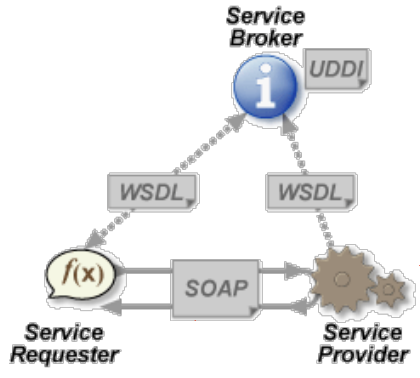
\includegraphics[width=\textwidth,keepaspectratio]{w3c_web_interactions}
    \end{figure}
\end{minipage}

\subsubsection*{Criticism of W3C}

\begin{enumerate}
    \item Too complex and intricate to fully implement
    \item Use of XML and SOAP lead to poor performance (HTTP is only used as a transport layer, services descriptions and invocations are very verbose)
    \item Service brokerage not really useful in practice (Developers know which service provider they want to connect to, rather than using any (unknown) service provider that happens to match a specification)
    \item Failure to impose open standards led to a plethora of proprietary, closed solutions
\end{enumerate}

\subsection{REST}

REST stand for Representational State Transfer. It was introduced in early 2000s. This is a general guidelines for designing Web architecture (best practices : not a formal standardized protocol, bottom-up normalization (rather than top-down)). The initial outcomes are HTTP 1.21 and URI (Uniform Resource Identifier). Compare to W3C WS, REST Web services use HTTP more directly.

\textbf{Key features}: Resources based, Representations and 6 constraints : uniform interface,
statelessness, client-server, cacheable, layered system and code on demand.

\subsubsection{Resources-based}

Deal with ’things’ rather than ’actions’ : REST over HTTP calls a thing (resource) and applies a HTTP verb to that thing whereas SOAP uses identified method calls (actions). It is ten easier to determine impact on architecture of a call with a given verb. Moreover each thing identified by one (or more) URI and a thing is separate from its representations (multiple representations possible for the same thing).

\subsubsection{Uniform Resource Identifier}

\begin{figure}[H]
    \centering
    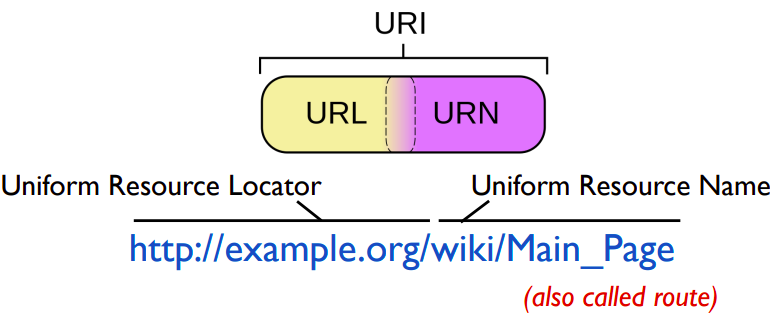
\includegraphics[width=0.8\textwidth,keepaspectratio]{uri}
\end{figure}

\subsubsection{Representations}

How resources are manipulated when exchanged between client/server (how they are stored by either party does not matter). Example : resource (student : john), service (personal information via GET) $\Rightarrow$ representation : name, program, list of pairs ¡course, grade¿ in a JSON or XML format.

\chapter{Storage}

\chapter{Elasticity green}

\section{Scaling}

\section{Elasticity}

\section{Energy efficiency}

\chapter{Fault Tolerance \& Consistency}

\chapter{Advanced IaaS}

\chapter{Security}

\chapter{Big Data}

\chapter{Blockchain}
